\documentclass[11pt,a4paper]{article}
\usepackage{amsmath,amssymb,amsfonts}
\usepackage{geometry}
\usepackage{enumitem}
\usepackage{graphicx}
\geometry{margin=1in}

\title{An introduction to the Born-Oppenheimer approximation}
\date{October 16, 2026}
\author{Yann Bruere \\ (\text{yann.bruere@gmail.com})}

\begin{document}
\maketitle

\section{Abstract}
We consider a molecule composed of $N$ nuclei labeled by index $\alpha=(1..N)$ and $K$ electrons labeled by index $i=(1..K)$. Solving the Schrödinger equation for molecules is extremely challenging because of the sheer number of variables. Indeed, each electron and nucleus having a 3D position, the number of variables in the molecular wave function is astronomically large. Instead of solving Schrödinger’s equation simultaneously for all these variables, the Born-Oppenheimer approximation calculates the electronic wave function by considering the nuclear positions as fixed parameters \cite{Born1927}. This is justified by the fact that nuclei are significantly heavier than electrons, and therefore nuclei move at very low speeds compared to electrons. In this approximation, the movement of nuclei is sufficiently slow to allow electrons to instantaneously adapt to changing nuclear configurations. Said differently, as nuclei move around the system remains in the same instantaneous electronic eigenstate without undergoing transitions to other states. This is the essence of the Adiabatic Theorem, which we will demonstrate in the first section of this paper. Once the wave functions for the fast-moving electrons are determined, the complete molecular state can be projected on the orthogonal basis of electronic energy eigenstates.

\section{Notations and definitions}
\begin{itemize}[label={}, leftmargin=*, itemsep=3pt, parsep=3pt]
    \item $e$ : elementary electric charge
    \item $\hbar$ : reduced Planck constant
    \item $\varepsilon_0$ : vacuum permittivity
    \item $m_e$ : electron rest mass
    \item $m_p$ : proton rest mass
    \item $m_\alpha$ : rest mass of nucleus $\alpha$
    \item $Z_\alpha$ : atomic number of nucleus $\alpha$
    \item $\mathrm{x}_i$ : 3D position vector of electron $i$
    \item $\mathbf{x}=(\mathrm{x}_1,\cdots,\mathrm{x}_K)$ concatenates the position vectors of the $K$ electrons
    \item $\mathbf{X}_\alpha$ : 3D position vector of nucleus $\alpha$
    \item $\mathbf{X}=(\mathrm{X}_1,\cdots,\mathrm{X}_N)$ concatenates the position vectors of the $N$ nuclei
    \item $\nabla_i = \left(\frac{\partial}{\partial x_i}, \frac{\partial}{\partial y_i}, \frac{\partial}{\partial z_i}\right)$ : gradient operator with respect to the position of electron $i$
    \item $\nabla_\alpha = \left(\frac{\partial}{\partial x_\alpha}, \frac{\partial}{\partial y_\alpha}, \frac{\partial}{\partial z_\alpha}\right)$ : gradient operator with respect to the position of nucleus $\alpha$
\end{itemize}

\section{The adiabatic theorem}\label{sec:The adiabatic theorem}
In thermodynamics, an \emph{adiabatic} process is one where no heat is exchanged with the boundary. The term comes from the Greek word \emph{adiabatos} that loosely translates to ‘no crossing’ which, in that context, means that no heat crosses the system-environment boundary. In quantum mechanics, an adiabatic process has a similar spirit: the Hamiltonian evolves sufficiently slowly that the system does not undergo transitions between different instantaneous energy eigenstates. We consider a system with a time-dependent Hamiltonian for which the Schrödinger equation is:
\begin{equation}
\label{eq:TDSE}
i\hbar \frac{\partial}{\partial t} |\psi(t)\rangle = H(t)|\psi(t)\rangle
\end{equation}
Each instant $t$ is associated with an \emph{instantaneous} energy eigenvalue equation:
\begin{equation}
\label{eq:Electronic eigenvalue equation}
H(t)|\psi_n(t)\rangle = E_n(t)|\psi_n(t)\rangle
\end{equation}
where $|\psi_n(t)\rangle$ is the instantaneous eigenstate corresponding to the $n$-th energy level denoted $E_n(t)$. It is important to bear in mind that numerical value for $n$-th energy level varies with time. Since $H(t)$ is an Hermitian operator, its instantaneous eigenstates form an orthonormal basis of the system’s Hilbert space. We can therefore decompose any state $|\psi(t)\rangle$ in this instantaneous basis (for simplicity, and without losing too much generality, the energy spectrum is assumed to be discrete and non-degenerate):
\begin{equation*}
	|\psi(t)\rangle = \sum_n a_n(t) |\psi_n(t)\rangle \quad \text{with } a_n(t) \in \mathbb{C}
\end{equation*}
Since the coefficient $a_n(t)$ are complex numbers we can always factor out an overall phase of our choosing such that:
\begin{equation*}
	a_n(t) = b_n(t) e^{i\theta_n(t)} \quad \text{with } \theta_n(t) \in \mathbb{R}
\end{equation*}
Our general state decomposition then becomes
\begin{equation*}
	\left|\psi(t)\right\rangle = \sum_n b_n(t) e^{i\theta_n(t)} \left|\psi_n(t)\right\rangle
\end{equation*}
For reasons that will become clear later, we define this overall factor to be (note that we have a different  phase factor for each energy level):
\begin{equation}
	\label{eq:Phase factor}
	\theta_n(t) = -\frac{1}{\hbar} \int_0^t E_n(t') \, dt'
\end{equation}
If we insert our $|\psi(t)\rangle$ decomposition into Schrodinger’s equation \eqref{eq:TDSE} we get:
\begin{equation*}
	\begin{gathered}
		i\hbar \frac{\partial}{\partial t} \left( \sum_n b_n(t) e^{i\theta_n(t)} \left|\psi_n(t)\right\rangle \right) = H(t) \sum_n b_n(t) e^{i\theta_n(t)} \left|\psi_n(t)\right\rangle \\[6pt]
		i\hbar \sum_n \left( \frac{\partial b_n}{\partial t} e^{i\theta_n(t)} \left|\psi_n(t)\right\rangle + b_n(t) i \frac{\partial \theta_n}{\partial t} e^{i\theta_n(t)} \left|\psi_n(t)\right\rangle \right. \\
		\left. + \, b_n(t) e^{i\theta_n(t)} \frac{\partial \left|\psi_n\right\rangle}{\partial t} \right) = \sum_n b_n(t) e^{i\theta_n(t)} H(t) \left|\psi_n(t)\right\rangle
	\end{gathered}
\end{equation*}
$|\psi_n(t)\rangle$ is an instantaneous eigenstate of $H(t)$ that follows equation \eqref{eq:Electronic eigenvalue equation}. Also, given our choice for the overall phase factor in equation \eqref{eq:Phase factor} we have:
\begin{equation*}
	\frac{\partial \theta_n}{\partial t} = \frac{\partial}{\partial t} \left( -\frac{1}{\hbar} \int_0^t E_n(t') \, dt' \right) = -\frac{E_n(t)}{\hbar}
\end{equation*}
The Schrödinger equation becomes:
\begin{equation*}
	\begin{gathered}
		i\hbar \sum_n \left( \frac{\partial b_n}{\partial t} e^{i\theta_n(t)} \left|\psi_n(t)\right\rangle + b_n(t) i \left(-\frac{E_n(t)}{\hbar}\right) e^{i\theta_n(t)} \left|\psi_n(t)\right\rangle + b_n(t) e^{i\theta_n(t)} \frac{\partial \left|\psi_n\right\rangle}{\partial t} \right) \\
		= \sum_n b_n(t) e^{i\theta_n(t)} E_n(t) \left|\psi_n(t)\right\rangle \\[6pt]
		i\hbar \sum_n \left( \frac{\partial b_n}{\partial t} e^{i\theta_n(t)} \left|\psi_n(t)\right\rangle + b_n(t) e^{i\theta_n(t)} \frac{\partial \left|\psi_n\right\rangle}{\partial t} \right) + \sum_n b_n(t) e^{i\theta_n(t)} E_n(t) \left|\psi_n(t)\right\rangle \\
		= \sum_n b_n(t) e^{i\theta_n(t)} E_n(t) \left|\psi_n(t)\right\rangle \\[6pt]
		\sum_n \frac{\partial b_n}{\partial t} e^{i\theta_n(t)} \left|\psi_n(t)\right\rangle = -\sum_n b_n(t) e^{i\theta_n(t)} \frac{\partial \left|\psi_n\right\rangle}{\partial t}
	\end{gathered}
\end{equation*}
We now take the scalar product with an instantaneous energy eigenstate $|\psi_m(t)\rangle$:
\begin{equation*}
	\begin{gathered}
		\langle \psi_m(t) | \sum_n \frac{\partial b_n}{\partial t} e^{i\theta_n(t)} \left|\psi_n(t)\right\rangle = -\langle \psi_m(t) | \sum_n b_n(t) e^{i\theta_n(t)} \frac{\partial \left|\psi_n(t)\right\rangle}{\partial t} \\[6pt]
		\sum_n \frac{\partial b_n}{\partial t} e^{i\theta_n(t)} \langle \psi_m(t) | \psi_n(t) \rangle = -\sum_n b_n(t) e^{i\theta_n(t)} \langle \psi_m(t) | \frac{\partial \left|\psi_n(t)\right\rangle}{\partial t}
	\end{gathered}
\end{equation*}
The instantaneous energy eigenstates are orthonormal and therefore $\langle \psi_m(t) | \psi_n(t) \rangle = \delta_{mn}$
\begin{equation*}
	\begin{gathered}
		\sum_n \frac{\partial b_n}{\partial t} e^{i\theta_n(t)} \delta_{mn} = -\sum_n b_n(t) e^{i\theta_n(t)} \langle \psi_m(t) | \frac{\partial \left|\psi_n(t)\right\rangle}{\partial t} \\[6pt]
		\frac{\partial b_m}{\partial t} = -\sum_n b_n(t) e^{i(\theta_n(t) - \theta_m(t))} \langle \psi_m(t) | \frac{\partial \left|\psi_n(t)\right\rangle}{\partial t}
	\end{gathered}
\end{equation*}
\begin{equation}
	\label{eq:Coef variation}
	\frac{\partial b_m}{\partial t} = -b_m(t) \langle \psi_m(t) | \frac{\partial \left|\psi_m(t)\right\rangle}{\partial t} - \sum_{n \neq m} b_n(t) e^{i(\theta_n(t) - \theta_m(t))} \langle \psi_m(t) | \frac{\partial \left|\psi_n(t)\right\rangle}{\partial t}
\end{equation}
In the last equation we have simply singled out the $n=m$ term of the sum. The $\langle \psi_m(t) | \frac{\partial \left|\psi_n(t)\right\rangle}{\partial t}$ term can be simplified by differentiating the instantaneous energy eigenvalue equation \eqref{eq:Electronic eigenvalue equation}, and then taking the scalar product with the instantaneous energy eigenstate $|\psi_m(t)\rangle$ distinct from $|\psi_n(t)\rangle$ (i.e. $n\neq m$).
\begin{equation*}
	\begin{gathered}
		\frac{\partial}{\partial t} \left( H(t) \left|\psi_n(t)\right\rangle \right) = \frac{\partial}{\partial t} \left( E_n(t) \left|\psi_n(t)\right\rangle \right) \\[6pt]
		\frac{\partial H(t)}{\partial t} \left|\psi_n(t)\right\rangle + H(t) \frac{\partial \left|\psi_n\right\rangle}{\partial t} = \frac{\partial E_n(t)}{\partial t} \left|\psi_n(t)\right\rangle + E_n(t) \frac{\partial \left|\psi_n(t)\right\rangle}{\partial t} \\[6pt]
		\langle \psi_m(t) | \frac{\partial H(t)}{\partial t} | \psi_n(t) \rangle + \langle \psi_m(t) | H(t) \frac{\partial \left|\psi_n\right\rangle}{\partial t} = \langle \psi_m(t) | \frac{\partial E_n(t)}{\partial t} | \psi_n(t) \rangle + \langle \psi_m(t) | E_n(t) \frac{\partial \left|\psi_n(t)\right\rangle}{\partial t} \\[6pt]
		\langle \psi_m(t) | \frac{\partial H(t)}{\partial t} | \psi_n(t) \rangle + E_m(t) \langle \psi_m(t) | \frac{\partial \left|\psi_n\right\rangle}{\partial t} = \delta_{mn} \frac{\partial E_n(t)}{\partial t} + E_n(t) \langle \psi_m(t) | \frac{\partial \left|\psi_n(t)\right\rangle}{\partial t}
	\end{gathered}
\end{equation*}
Because $n\neq m$ we have $\delta_{mn}=0$ and therefore:
\begin{equation*}
	\langle \psi_m(t) | \frac{\partial \left|\psi_n(t)\right\rangle}{\partial t} = \frac{\langle \psi_m(t) | \frac{\partial H(t)}{\partial t} | \psi_n(t) \rangle}{E_n(t) - E_m(t)}
\end{equation*}
Finally, replacing in equation \eqref{eq:Coef variation} yields the rate of change of coefficient $b_m$
\begin{equation*}
	\frac{\partial b_m}{\partial t} = -b_m(t) \langle \psi_m(t) | \frac{\partial \left|\psi_m(t)\right\rangle}{\partial t} - \sum_{n \neq m} b_n(t) e^{i(\theta_n(t) - \theta_m(t))} \frac{\langle \psi_m(t) | \frac{\partial H(t)}{\partial t} | \psi_n(t) \rangle}{E_n(t) - E_m(t)}
\end{equation*}
If the Hamiltonian varies relatively slowly with time and the instantaneous discrete energy levels are sufficiently spread out, then the ratio of $\langle \psi_m(t) | \frac{\partial H(t)}{\partial t} | \psi_n(t) \rangle$ over $E_n(t) - E_m(t)$ becomes negligible. In this adiabatic limit we are thus left with:
\begin{equation*}
	\frac{\partial b_m}{\partial t} = -b_m(t) \langle \psi_m(t) | \frac{\partial \left|\psi_m(t)\right\rangle}{\partial t}
\end{equation*}
\begin{equation}
	\label{eq:Coef equation}
	\Rightarrow b_m(t) = b_m(0) \exp\left( -\int^t \langle \psi_m(t') | \frac{\partial |\psi_m(t')\rangle}{\partial t'} \, dt' \right)
\end{equation}
Because our electronic energy eigenstates are normalized we have:
\begin{equation*}
	\begin{gathered}
		\langle \psi_m(t) | \psi_m(t) \rangle = 1 \\[6pt]
		\frac{\partial}{\partial t} \left( \langle \psi_m(t) | \psi_m(t) \rangle \right) = 0 \\[6pt]
		\frac{\partial \langle \psi_m(t) |}{\partial t} \left|\psi_m(t)\right\rangle + \langle \psi_m(t) | \frac{\partial \left|\psi_m(t)\right\rangle}{\partial t} = 0 \\[6pt]
		\left( \langle \psi_m(t) | \frac{\partial \left|\psi_m(t)\right\rangle}{\partial t} \right)^* + \langle \psi_m(t) | \frac{\partial \left|\psi_m(t)\right\rangle}{\partial t} = 0
	\end{gathered}
\end{equation*}
The last equation means that $\langle \psi_m(t) | \frac{\partial \left|\psi_m(t)\right\rangle}{\partial t}$ is a pure imaginary number such that:
\begin{equation*}
	\langle \psi_m(t) | \frac{\partial \left|\psi_m(t)\right\rangle}{\partial t} = i \boldsymbol{\mathcal{A}}_n(t) \quad (\boldsymbol{\mathcal{A}}_n \in \mathbb{R})
\end{equation*}
$\boldsymbol{\mathcal{A}}_n$ is called the \emph{Berry connection} (more on this in the next section). Equation \eqref{eq:Coef equation} can then be rewritten as
\begin{equation}
	\label{eq:Berry phase}
	b_m(t) = b_m(0) \exp\left( -i \int^t \boldsymbol{\mathcal{A}}_n(t') \, dt' \right)
\end{equation}
Suppose we initially start with the system exactly in a definite energy eigenstate $\left|\psi_n\right\rangle$ with:
\begin{equation*}
	b_n(t=0) = 1 \quad \text{and} \quad b_m(t=0) = 0 \quad \text{for } m \neq n
\end{equation*}
Since we have set the initial system configuration such that $b_m(t=0) = 0$ for $m \neq n$, equation \eqref{eq:Berry phase} tells us that $b_m(t)$ remains zero at later times. In plain English this means that if the system starts in instantaneous eigenstate $\left|\psi_n(t=0)\right\rangle$, it will remain in the same \emph{instantaneous} eigenstate $\left|\psi_n(t)\right\rangle$ at later time.

\section{The Born-Oppenheimer approximation}
The complete molecular state $\left|\Psi\right\rangle$ lives in the tensor product of the nuclear and electronic Hilbert spaces $\mathcal{H} = \mathcal{H}_{\text{elec}} \otimes \mathcal{H}_{\text{nucl}}$. The molecular wave function expanded in the $\left|\mathbf{x}\right\rangle \otimes \left|\mathbf{X}\right\rangle$ product basis is
\begin{equation*}
	\Psi(\mathbf{x}, \mathbf{X}) = \left(\langle\mathbf{x}| \otimes \langle\mathbf{X}|\right) \left|\Psi\right\rangle
\end{equation*}
The ket $\left|\phi(\mathbf{X})\right\rangle$ is the electronic quantum state when the nuclei are at positions $\mathbf{X}$. For a given nuclei positions configuration $\mathbf{X}$, the electronic Hamiltonian is an Hermitian operator whose eigenstates form an orthogonal basis of the electronic Hilbert space. We will write $\left|\phi_n(\mathbf{X})\right\rangle$ the electronic energy eigenstates when the positions of nuclei is $\mathbf{X}$ (the $n$ subscript refers to the $n$-th energy level):
\begin{equation}
	\label{eq:Nuclear electronic eigenvalue equation}
	H_{el}(\mathbf{X}) \left|\phi_n(\mathbf{X})\right\rangle = E_n^{el}(\mathbf{X}) \left|\phi_n(\mathbf{X})\right\rangle
\end{equation}
where $H_{el}(X)$ is the electronic Hamiltonian when the nuclei position is $\mathbf{X}$. The resolution of the identity for these electronic energy eigenstates is:
\begin{equation*}
	\sum_n |\phi_n(\mathbf{X})\rangle \langle\phi_n(\mathbf{X})| = \mathbf{1}
\end{equation*}
We can insert this resolution of the identify into the definition of $\Psi(\mathbf{x},\mathbf{X})$
\begin{equation*}
	\begin{gathered}
		\Psi(\mathbf{x}, \mathbf{X}) = (\langle\mathbf{x}| \otimes \langle\mathbf{X}|) \left( \sum_n |\phi_n(\mathbf{X})\rangle \langle\phi_n(\mathbf{X})| \right) |\Psi\rangle \\[6pt]
		\Psi(\mathbf{x}, \mathbf{X}) = \sum_n \langle\mathbf{x} | \phi_n(\mathbf{X})\rangle \langle\mathbf{X}| (\langle\phi_n(\mathbf{X})|\Psi\rangle)
	\end{gathered}
\end{equation*}
The $\langle\mathbf{x} | \phi_n(\mathbf{X})\rangle$ term is the electronic wave function expressed in the electrons position basis $|\mathbf{x}\rangle$:
\begin{equation*}
	\langle\mathbf{x} | \phi_n(\mathbf{X})\rangle = \phi_n(\mathbf{x}; \mathbf{X})
\end{equation*}
The other term $\langle\phi_n(\mathbf{X}) | \Psi\rangle$ is the projection of the molecular state $\left|\Psi\right\rangle$ on the electronic eigenstate $\left|\phi_n(\mathbf{X})\right\rangle$. Since $\langle\phi_n(\mathbf{X}) | \Psi\rangle$ lives in the $\mathcal{H}_{\text{elec}} \otimes \mathcal{H}_{\text{nucl}}$ product space, once you project it onto an electronic Hilbert space you are left with an object that lives in the nuclear Hilbert space. This object is analogous to a nuclear quantum state which we will write $|\Phi_n\rangle$:
\begin{equation*}
	|\Phi_n\rangle = \langle\phi_n(\mathbf{X}) | \Psi\rangle
\end{equation*}
Its projection on a nuclei position eigenstate $|\mathbf{X}\rangle$ is simply the nuclear wave function $\Phi_n(\mathbf{X})$ associated with the electronic $n$-th energy level:
\begin{equation*}
	\langle\mathbf{X} | (\langle\phi_n(\mathbf{X}) | \Psi\rangle) = \langle\mathbf{X} | \Phi_n\rangle = \Phi_n(\mathbf{X}) 
\end{equation*}
After inserting these results in the molecular wave function equation we get:
\begin{equation*}
	\Psi(\mathbf{x}, \mathbf{X}) = \sum_n \phi_n(\mathbf{x}; \mathbf{X}) \Phi_n(\mathbf{X})
\end{equation*}
and the molecular energy eigenvalue equation is
\begin{equation}
	\label{eq:Molecular energy eigenvalue equation}
	(H_{nucl}(\mathbf{X}) + H_{el}(\mathbf{X})) \Psi(\mathbf{x}, \mathbf{X}) = E \Psi(\mathbf{x}, \mathbf{X})
\end{equation}
where $H_{nucl}$ and $H_{el}$ are the nuclear and electronic Hamiltonians, respectively.

\subsection{Effective nuclear potential energy}
We would like to find the effective nuclear Hamiltonian such that:
\begin{equation*}
	H_{nucl}^n(\mathbf{X}) \Phi_n(\mathbf{X}) = E \Phi_n(\mathbf{X})
\end{equation*}
In other words, we are looking for the Hamiltonian that links the total molecular energy with the nuclear quantum state $|\Phi_n\rangle$. We start by inserting the $\Psi(\mathbf{x}, \mathbf{X}) = \sum_n \phi_n(\mathbf{x}; \mathbf{X}) \Phi_n(\mathbf{X})$ expansion into equation \eqref{eq:Molecular energy eigenvalue equation}:
\begin{equation*}
	\begin{gathered}
		H_{nucl} \sum_n |\phi_n\rangle \Phi_n + H_{el} \sum_n |\phi_n\rangle \Phi_n = E \sum_n |\phi_n\rangle \Phi_n \\[6pt]
		\sum_n H_{nucl} (|\phi_n\rangle \Phi_n) + \sum_n H_{el} |\phi_n\rangle \Phi_n = E \sum_n |\phi_n\rangle \Phi_n \\[6pt]
		\sum_n H_{nucl} (|\phi_n\rangle \Phi_n) + \sum_n E_n^{el} |\phi_n\rangle \Phi_n = E \sum_n |\phi_n\rangle \Phi_n \\[6pt]
		\sum_n \langle\phi_m | H_{nucl} (|\phi_n\rangle \Phi_n) + \sum_n E_n^{el} \langle\phi_m | \phi_n\rangle \Phi_n = E \sum_n \langle\phi_m | \phi_n\rangle \Phi_n \\[6pt]
		\sum_n \langle\phi_m | H_{nucl} (|\phi_n\rangle \Phi_n) + \sum_n E_n^{el} \delta_{nm} \Phi_n = E \sum_n \delta_{nm} \Phi_n
	\end{gathered}
\end{equation*}
\begin{equation}
	\label{eq:Raw effective nuclear energy}
	\sum_n \langle\phi_m | H_{nucl} (|\phi_n\rangle \Phi_n) + E_m^{el} \Phi_m = E \Phi_m
\end{equation}
The nuclear Hamiltonian consists of the nuclei kinetic energy and the Coulomb repulsion potential between nuclei (the $1/2$ factor in front of the Coulomb repulsion term is necessary to avoid counting inter-nuclei interactions twice):
\begin{equation*}
	\begin{gathered}
		H_{nucl} = -\sum_\alpha \frac{\hbar^2}{2m_\alpha} \nabla_\alpha^2 + \frac{1}{2} \frac{e^2}{4\pi\varepsilon_0} \sum_{\alpha \neq \beta} \frac{Z_\alpha Z_\beta}{|\mathbf{X}_\alpha - \mathbf{X}_\beta|} \\[6pt]
		\Rightarrow \langle\phi_m | H_{nucl} (|\phi_n\rangle \Phi_n) = -\sum_\alpha \frac{\hbar^2}{2m_\alpha} \langle\phi_m | \nabla_\alpha^2 (|\phi_n\rangle \Phi_n) + \frac{e^2}{8\pi\varepsilon_0} \langle\phi_m | \sum_{\alpha \neq \beta} \frac{Z_\alpha Z_\beta}{|\mathbf{X}_\alpha - \mathbf{X}_\beta|} |\phi_n\rangle \Phi_n
	\end{gathered}
\end{equation*}
Since $\nabla_\alpha^2$ is the Laplacian operator with respect to the position of nucleus $\alpha$, it impacts both the nuclear and electronic wave functions. We thus write
\begin{equation*}
	\langle\phi_m | H_{nucl} (|\phi_n\rangle \Phi_n) = -\sum_\alpha \frac{\hbar^2}{2m_\alpha} \langle\phi_m | \nabla_\alpha^2 (|\phi_n\rangle \Phi_n) + \frac{e^2}{8\pi\varepsilon_0} \sum_{\alpha \neq \beta} \frac{Z_\alpha Z_\beta}{|\mathbf{X}_\alpha - \mathbf{X}_\beta|} \delta_{nm} \Phi_n
\end{equation*}
which inserted in equation \eqref{eq:Raw effective nuclear energy} yields
\begin{equation*}
	\begin{gathered}
		\sum_n \left( -\sum_\alpha \frac{\hbar^2}{2m_\alpha} \langle\phi_m | \nabla_\alpha^2 (|\phi_n\rangle \Phi_n) + \frac{e^2}{8\pi\varepsilon_0} \sum_{\alpha \neq \beta} \frac{Z_\alpha Z_\beta}{|\mathbf{X}_\alpha - \mathbf{X}_\beta|} \delta_{nm} \Phi_n \right) + E_m^{el} \Phi_m = E \Phi_m \\[6pt]
		-\sum_n \left( \sum_\alpha \frac{\hbar^2}{2m_\alpha} \langle\phi_m | \nabla_\alpha^2 (|\phi_n\rangle \Phi_n) \right) + \sum_n \left( \frac{e^2}{8\pi\varepsilon_0} \sum_{\alpha \neq \beta} \frac{Z_\alpha Z_\beta}{|\mathbf{X}_\alpha - \mathbf{X}_\beta|} \delta_{nm} \Phi_n \right) + E_m^{el} \Phi_m = E \Phi_m
	\end{gathered}
\end{equation*}
\begin{equation}
	\label{eq:Raw effective nuclear energy bis}
	-\sum_n \left( \sum_\alpha \frac{\hbar^2}{2m_\alpha} \langle\phi_m | \nabla_\alpha^2 (\Phi_n |\phi_n\rangle) \right) + \frac{e^2}{8\pi\varepsilon_0} \sum_{\alpha \neq \beta} \frac{Z_\alpha Z_\beta}{|\mathbf{X}_\alpha - \mathbf{X}_\beta|} \Phi_m + E_m^{el} \Phi_m = E \Phi_m
\end{equation}
We first evaluate the matrix element $\langle\phi_m | \nabla_\alpha^2 (\Phi_n |\phi_n\rangle)$
\begin{equation*}
	\begin{gathered}
		\nabla_\alpha (\Phi_n(\mathbf{X}) |\phi_n(\mathbf{x}; \mathbf{X})\rangle) = \nabla_\alpha \Phi_n(\mathbf{X}) |\phi_n(\mathbf{x}; \mathbf{X})\rangle + \nabla_\alpha |\phi_n(\mathbf{x}; \mathbf{X})\rangle \Phi_n(\mathbf{X}) \\[6pt]
		\nabla_\alpha^2 (\Phi_n |\phi_n\rangle) = \nabla_\alpha^2 \Phi_n |\phi_n\rangle + \nabla_\alpha \Phi_n \nabla |\phi_n\rangle + \nabla_\alpha^2 |\phi_n\rangle \Phi_n + \nabla_\alpha |\phi_n\rangle \nabla\Phi_n \\[6pt]
		\nabla_\alpha^2 (\Phi_n |\phi_n\rangle) = \nabla_\alpha^2 \Phi_n |\phi_n\rangle + 2 \nabla_\alpha |\phi_n\rangle \nabla_\alpha \Phi_n + \nabla_\alpha^2 |\phi_n\rangle \Phi_n
	\end{gathered}
\end{equation*}
\begin{equation}
	\label{eq:Laplacian expansion}
	\langle\phi_m | \nabla_\alpha^2 (\Phi_n |\phi_n\rangle) = \left( \delta_{nm} \nabla_\alpha^2 + 2\langle\phi_m | \nabla_a | \phi_n\rangle \nabla_\alpha + \langle\phi_m | \nabla_\alpha^2 | \phi_n\rangle \right) \Phi_n
\end{equation}
The $\langle\phi_m | \nabla_\alpha^2 | \phi_n\rangle$ term can be massaged into something containing only first order derivatives:
\begin{equation*}
	\begin{gathered}
		\nabla_\alpha (\langle\phi_m | \nabla_\alpha | \phi_n\rangle) = \nabla_\alpha (\langle\phi_m |) \nabla_\alpha |\phi_n\rangle + \langle\phi_m | \nabla_\alpha^2 | \phi_n\rangle \\[6pt]
		\langle\phi_m | \nabla_\alpha^2 | \phi_n\rangle = \nabla_\alpha (\langle\phi_m | \nabla_\alpha | \phi_n\rangle) - \nabla_\alpha (\langle\phi_m |) \nabla_\alpha |\phi_n\rangle \\[6pt]
		\langle\phi_m | \nabla_\alpha^2 | \phi_n\rangle = \nabla_\alpha (\langle\phi_m | \nabla_\alpha | \phi_n\rangle) - \nabla_\alpha (\langle\phi_m |) \left(\sum_l |\phi_l\rangle \langle\phi_l|\right) \nabla_\alpha |\phi_n\rangle \\[6pt]
		\langle\phi_m | \nabla_\alpha^2 | \phi_n\rangle = \nabla_\alpha (\langle\phi_m | \nabla_\alpha | \phi_n\rangle) - \sum_l \nabla_\alpha (\langle\phi_m |) |\phi_l\rangle \langle\phi_l | \nabla_\alpha | \phi_n\rangle
	\end{gathered}
\end{equation*}
We can easily show that $\nabla_\alpha (\langle\phi_m |) |\phi_n\rangle = -\langle\phi_m | \nabla_\alpha | \phi_n\rangle$. Indeed:
\begin{equation*}
	\begin{gathered}
		\nabla_\alpha (\langle\phi_m | \phi_n\rangle) = \nabla_\alpha (\delta_{nm}) = 0 = \nabla_\alpha (\langle\phi_m |) |\phi_n\rangle + \langle\phi_m | \nabla_\alpha | \phi_n\rangle \\[6pt]
		\Rightarrow \nabla_\alpha (\langle\phi_m |) |\phi_n\rangle = -\langle\phi_m | \nabla_\alpha | \phi_n\rangle \\[6pt]
		\Rightarrow \langle\phi_m | \nabla_\alpha^2 | \phi_n\rangle = \nabla_\alpha (\langle\phi_m | \nabla_\alpha | \phi_n\rangle) + \sum_l \langle\phi_m | \nabla_\alpha | \phi_l\rangle \langle\phi_l | \nabla_\alpha | \phi_n\rangle
	\end{gathered}
\end{equation*}
We can replace this expression for $\langle\phi_m | \nabla_\alpha^2 (\Phi_n |\phi_n\rangle)$ in equation \eqref{eq:Laplacian expansion} to get
\begin{equation*}
	\begin{split}
		\langle\phi_m | \nabla_\alpha^2 (\Phi_n |\phi_n\rangle) = & \Big[ \delta_{nm} \nabla_\alpha^2 + 2\langle\phi_m | \nabla_\alpha | \phi_n\rangle \nabla_\alpha + \nabla_\alpha(\langle\phi_m | \nabla_\alpha | \phi_n\rangle) \\
		& + \sum_l \langle\phi_m | \nabla_\alpha | \phi_l\rangle \langle\phi_l | \nabla_\alpha | \phi_n\rangle \Big] \Phi_n
	\end{split}
\end{equation*}
Looking at equation \eqref{eq:Raw effective nuclear energy bis} we see that we must calculate the sum over $n$ of the previous equation:
\begin{equation*}
	\begin{split}
		\sum_n \langle\phi_m | \nabla_\alpha^2 (\Phi_n |\phi_n\rangle) = \sum_n & \Big[ \delta_{nm} \nabla_\alpha^2 + 2\langle\phi_m | \nabla_\alpha | \phi_n\rangle \nabla_\alpha + \nabla_\alpha(\langle\phi_m | \nabla_\alpha | \phi_n\rangle) \\
		& + \sum_l \langle\phi_m | \nabla_\alpha | \phi_l\rangle \langle\phi_l | \nabla_\alpha | \phi_n\rangle \Big] \Phi_n
	\end{split}
\end{equation*}
which if we isolate the $n=m$ term becomes
\begin{equation*}
	\begin{split}
		& \Big( \nabla_\alpha^2 + 2\langle\phi_m | \nabla_\alpha | \phi_m\rangle \nabla_\alpha + \nabla_\alpha(\langle\phi_m | \nabla_\alpha | \phi_m\rangle) + \sum_l \langle\phi_m | \nabla_\alpha | \phi_l\rangle \langle\phi_l | \nabla_\alpha | \phi_m\rangle \Big) \Phi_m \\
		& + \sum_{n \neq m} \Big( 2\langle\phi_m | \nabla_\alpha | \phi_n\rangle \nabla_\alpha + \nabla_\alpha(\langle\phi_m | \nabla_\alpha | \phi_n\rangle) + \sum_l \langle\phi_m | \nabla_\alpha | \phi_l\rangle \langle\phi_l | \nabla_\alpha | \phi_n\rangle \Big) \Phi_n
	\end{split}
\end{equation*}
We now show that the sum over $n \neq m$ is null because, in the adiabatic limit, $\langle\phi_m | \nabla_\alpha | \phi_n\rangle = 0$. To do so we apply the $\nabla_{\alpha}$ operator to the eigenvalue equation \eqref{eq:Nuclear electronic eigenvalue equation}:
\begin{equation*}
	\begin{gathered}
		\nabla_\alpha (H_{el} |\phi_n\rangle) = \nabla_\alpha (E_n^{el} |\phi_n\rangle) \\[6pt]
		\nabla_\alpha H_{el} |\phi_n\rangle + H_{el} \nabla_\alpha |\phi_n\rangle = \nabla_\alpha E_n^{el} |\phi_n\rangle + E_n^{el} \nabla_\alpha |\phi_n\rangle
	\end{gathered}
\end{equation*}
The scalar product with eigenstate $|\phi_m\rangle$ for $m \neq n$ yields:
\begin{equation*}
	\begin{gathered}
		\langle\phi_m | \nabla_\alpha H_{el} |\phi_n\rangle + \langle\phi_m | H_{el} \nabla_\alpha |\phi_n\rangle = \nabla_\alpha E_n^{el} \langle\phi_m \mid \phi_n\rangle + E_n^{el} \langle\phi_m | \nabla_\alpha |\phi_n\rangle \\[6pt]
		\langle\phi_m | \nabla_\alpha H_{el} |\phi_n\rangle + E_m^{el} \langle\phi_m | \nabla_\alpha |\phi_n\rangle = \nabla_\alpha E_n^{el} \delta_{mn} + E_n^{el} \langle\phi_m | \nabla_\alpha |\phi_n\rangle \\[6pt]
		\langle\phi_m | \nabla_\alpha |\phi_n\rangle = \frac{\langle\phi_m | \nabla_\alpha H_{el} |\phi_n\rangle}{E_n^{el} - E_m^{el}}
	\end{gathered}
\end{equation*}
In the adiabatic limit the variation of $H_{el}$ with respect to nucleus $\alpha$ position is very small compared to the difference between two electronic energy levels $E_n^{el}-E_m^{el}$. We thus have $\langle\phi_m | \nabla_\alpha |\phi_n\rangle = 0$ for $m \neq n$ which allows us to write
\begin{equation*}
	\begin{split}
		\sum_n \langle\phi_m | \nabla_\alpha^2 (\Phi_n |\phi_n\rangle) = & \Big( \nabla_\alpha^2 + 2\langle\phi_m | \nabla_\alpha | \phi_m\rangle \nabla_\alpha + \nabla_\alpha(\langle\phi_m | \nabla_\alpha | \phi_m\rangle) \\
		& + \sum_l \langle\phi_m | \nabla_\alpha | \phi_l\rangle \langle\phi_l | \nabla_\alpha | \phi_m\rangle \Big) \Phi_m \\[6pt]
		\Leftrightarrow \sum_n \langle\phi_m | \nabla_\alpha^2 (\Phi_n |\phi_n\rangle) = & \Big( (\nabla_\alpha + i\boldsymbol{\mathcal{A}}_{m,\alpha})^2 + \sum_{l \neq m} |\langle\phi_l | \nabla_\alpha | \phi_m\rangle|^2 \Big) \Phi_m
	\end{split}
\end{equation*}
where we recognize $\boldsymbol{\mathcal{A}}_{m,\alpha} = -i \langle\phi_m | \nabla_\alpha | \phi_m\rangle$ to be the Berry connection for nucleus $\alpha$.
We can insert this expression in equation \eqref{eq:Raw effective nuclear energy bis} and get
\begin{equation*}
	\begin{gathered}
		-\sum_\alpha \frac{\hbar^2}{2m_\alpha} \Big( (\nabla_\alpha + i\boldsymbol{\mathcal{A}}_{m,\alpha})^2 + \sum_{l \neq m} |\langle\phi_l | \nabla_\alpha | \phi_m\rangle|^2 \Big) \Phi_m + \frac{e^2}{8\pi\varepsilon_0} \sum_{\alpha \neq \beta} \frac{Z_\alpha Z_\beta}{|\mathbf{X}_\alpha - \mathbf{X}_\beta|} \Phi_m + E_m^{el} \Phi_m = E \Phi_m \\[6pt]
		\Leftrightarrow H_{nucl}^n(\mathbf{X}) \Phi_n = E \Phi_n
	\end{gathered}
\end{equation*}
$H_{nucl}^n$ is the \emph{effective nuclear Hamiltonian} associated with electronic energy eigenstate $|\phi_n\rangle$ defined as
\begin{equation}
	\label{eq:Effective nuclear Hamiltonian}
	H_{nucl}^n(\mathbf{X}) = -\sum_\alpha \frac{\hbar^2}{2m_\alpha} (\nabla_\alpha + i\boldsymbol{\mathcal{A}}_{n,\alpha})^2 + \frac{e^2}{8\pi\varepsilon_0} \sum_{\alpha \neq \beta} \frac{Z_\alpha Z_\beta}{|\mathbf{X}_\alpha - \mathbf{X}_\beta|} + E_n^{el}(\mathbf{X}) - \sum_\alpha \frac{\hbar^2}{2m_\alpha} W_{n,\alpha}(\mathbf{X})
\end{equation}
where we have introduced the notation $W_{n,\alpha}(\mathbf{X}) = \sum_{l \neq n} |\langle\phi_l | \nabla_\alpha | \phi_n\rangle|^2$. Let’s unpack the various terms present in equation \eqref{eq:Effective nuclear Hamiltonian}.

\subsubsection{Nuclear covariant derivative}
The $\frac{\hbar^2}{2m_\alpha} (\nabla_\alpha + i\boldsymbol{\mathcal{A}}_{n,\alpha})^2$ term is the momentum operator for nucleus $\alpha$. Compared to the classical momentum operator $\frac{\hbar^2}{2m_\alpha}\nabla_\alpha$ we see it includes the Berry connection $\boldsymbol{\mathcal{A}}_{n,\alpha}$ introduced at the end of section \ref{sec:The adiabatic theorem}. This correction, which was discarded in the original Born-Oppenheimer approximation, is kept intact in the subsequent Born-Huang approximation \cite{BornHuang1954}. The form $(\nabla_\alpha + i\boldsymbol{\mathcal{A}}_{n,\alpha})$ is eerily reminiscent of the generic definition of a covariant derivative $\boldsymbol{D} = \nabla + i\boldsymbol{\mathcal{A}}$, where $\boldsymbol{\mathcal{A}}$ acts as a \emph{connection} in differential geometry. For instance, in the quantum electrodynamic context, the connection is associated with the electromagnetic gauge field $\boldsymbol{\mathcal{A}} = (\phi,\vec{\mathcal{A}})$ where $\phi$ is the electric scalar potential, and $\vec{\mathcal{A}}$ is the magnetic vector potential. In the Born-Oppenheimer context, the Berry connection $\boldsymbol{\mathcal{A}}_{n,\alpha}$ acts similarly and accounts for the magnetic-like effect the surrounding electrons exert on the nuclei. Specifically, $\boldsymbol{\mathcal{A}}_{n,\alpha}$ acts as a gauge field that reveals how the momentum operator for nucleus $\alpha$ interacts with the electrons sitting in the $n$-th energy eigenstate. As nucleus $\alpha$ position slowly evolves with time, the electronic state shifts to another \emph{version} of the $n$-th instantaneous energy eigenstate. This in turn impacts the motion of the nucleus, which is what the extra $i\boldsymbol{\mathcal{A}}_{n,\alpha}$ term in the \emph{nuclear covariant momentum operator} accounts for. Mathematically, we say that the nuclear quantum state $|\Phi_n\rangle$ lives in the $3N$ manifold spanning the nuclei configuration space $\mathbf{X}=(\mathrm{X}_1,\cdots,\mathrm{X}_\alpha)$. At each point on the configuration space, the set of $|\phi_n(\mathbf{X})\rangle$ electronic energy eigenstates constitutes a local basis of this manifold. The Berry connection $\boldsymbol{\mathcal{A}}_{n,\alpha}$ tells us how the basis vector $|\phi_n(\mathbf{X})\rangle$ evolves when nucleus $\alpha$ is moved. The \emph{nuclear covariant derivative} $(\nabla_\alpha + i\boldsymbol{\mathcal{A}}_{n,\alpha})$ compensates for this curvature of the configuration space caused by cloud of electrons surrounding the nuclei.

\subsubsection{Effective nuclear potential energy}
The other terms in equation \eqref{eq:Effective nuclear Hamiltonian} are different flavors of potential energy. The first one is the classical inter-nuclear Coulomb repulsion potential energy:
\begin{equation*}
	\frac{e^2}{8\pi\varepsilon_0} \sum_{\alpha \neq \beta} \frac{Z_\alpha Z_\beta}{|\mathbf{X}_\alpha - \mathbf{X}_\beta|}
\end{equation*}
The second one $E_n^{el}$ is the electronic energy associated with eigenstate $|\phi_n\rangle$. Its values are derived from the electronic Hamiltonian eigenvalue equation \eqref{eq:Nuclear electronic eigenvalue equation}. The electronic Hamiltonian $H_{el}$ includes the electrons’ kinetic energy, the Coulomb repulsion potential between electrons (with the $1/2$ factor to avoid double counting), and the Coulomb attraction potential between electrons and the nuclei at fixed positions $\mathbf{X}=(\mathrm{X}_1,\cdots,\mathrm{X}_\alpha)$:
\begin{equation*}
	H_{el}(\mathbf{X}) = -\frac{\hbar^2}{2m_e} \sum_i \nabla_i^2 + \frac{1}{2} \frac{e^2}{4\pi\varepsilon_0} \sum_{i \neq j} \frac{1}{|\mathbf{x}_i - \mathbf{x}_j|} - \frac{e^2}{4\pi\varepsilon_0} \sum_{i,\alpha} \frac{Z_\alpha}{|\mathbf{X}_\alpha - \mathbf{x}_i|}
\end{equation*}
If the electrons were not present the potential energy would be limited to the inter-nuclei Coulomb repulsion. The $E_n^{el}(\mathbf{X})$ term is the quantum shift in nuclear potential energy induced by the presence of the electrons. It is often referred to as the \emph{Potential Energy Surface} in which the nuclei move.\\ The last term $W_{n,\alpha}(\mathbf{X}) = \sum_{l \neq n} |\langle\phi_l | \nabla_\alpha | \phi_n\rangle|^2$ is the \emph{Diagonal Adiabatic Correction}. To get some intuition about its physical meaning we can study its structure.  $\nabla_\alpha | \phi_n\rangle$ is the variation of electronic eigenstate $|\phi_n\rangle$ induced by the movement of nucleus $\alpha$. Its projection onto $|\phi_l\rangle$ tells us how much of this variation \emph{leaks} into another electronic eigenstate $|\phi_l\rangle$. Therefore, $\sum_{l \neq n} |\langle\phi_l | \nabla_\alpha | \phi_n\rangle|^2$ represents the total leakage from $n$ to other electronic states $l \neq n$ induced the movement of nucleus $\alpha$. In the Born-Oppenheimer model, even though the electrons stay in the same instantaneous energy eigenstate $n$, other electronic energy levels $l \neq n$ are somehow \emph{virtually} perturbed. This is responsible for yet another nuclear potential energy shift. In the classical two-body problem the centrifugal force is added to the gravitation potential to form the effective potential energy. The same logic is at play here; the electronic energy $E_n^{el}$ and the Diagonal Adiabatic Correction $W_{n,\alpha}$ are added to classical inter-nuclear Coulomb potential energy to form the complete \emph{effective nuclear potential energy}
\begin{equation}
	\label{eq:Effective nuclear potential energy}
	V_{\text{eff}}^n(\mathbf{X}) = \frac{e^2}{8\pi\varepsilon_0} \sum_{\alpha \neq \beta} \frac{Z_\alpha Z_\beta}{|\mathbf{X}_\alpha - \mathbf{X}_\beta|} + E_n^{el}(\mathbf{X}) - \sum_\alpha \frac{\hbar^2}{2m_\alpha} W_{n,\alpha}(\mathbf{X})
\end{equation}

\section{The $\text{H}_2^+$ molecular ion}
In this section we apply the Born-Oppenheimer approximation to the simplest of all molecules, the dihydrogen molecular ion which consists of two hydrogen nuclei sharing one electron. Each hydrogen nucleus has only one proton, so we have $Z_1 = Z_2 = 1$. Also, with only one electron, there is no inter-electron Coulomb repulsion to consider. The nuclei positions are given by position vectors $R_1=(x_1,y_1,z_1)$ and $R_2=(x_2,y_2,z_2)$, with their relative distance denoted $R=|R_1-R_2|$. Since the internuclear distance $R$ is the only degree of freedom,  $\text{H}_2^+$ nuclear configuration space is uni-dimensional.\\
We first calculate the wave function for the electronic energy eigenstates:
\begin{equation*}
	\begin{gathered}
		H_{el}(R) |\phi_n(R)\rangle = E_n^{el}(R) |\phi_n(R)\rangle \\[6pt]
		\left( -\frac{\hbar^2}{2m_e} \nabla_e^2 - \frac{e^2}{4\pi\varepsilon_0} \left( \frac{1}{|R_1 - \mathrm{x}|} + \frac{1}{|R_2 - \mathrm{x}|} \right) \right) \phi_n(\mathrm{x}, R) = E_n^{el}(R) \phi_n(\mathrm{x}, R)
	\end{gathered}
\end{equation*}
where $\nabla_e^2$ is the Laplacian operator with respect to the electron’s 3D position vector $\mathrm{x} = (x_e,y_e,z_e)$. There are several ways to solve this eigenvalue problem, like the \emph{Linear Combination of Atomic Orbitals} (LCAO) approach \cite{SzaboOstlund}. However, we will not attempt to find an analytic solution and instead resort to brute force numerical resolution to find the electronic eigenstates and energy levels. In that spirit, $\phi_n(\mathrm{x}, R)$ and $E_n^{el}(R)$ are computed for various values of internuclear distance R, and the latter is used to calculate the effective nuclear potential energy of $\text{H}_2^+$
\begin{equation*}
	V_{\text{eff}}^n(R) = \frac{e^2}{4\pi\varepsilon_0 R} + E_n^{el}(R) - \frac{\hbar^2}{2m_p} \sum_{l \neq n} W_{n,\alpha}(\mathbf{X})
\end{equation*}
The last term is the Diagonal Adiabatic Correction. Given that the proton rest mass is many times larger than the typical electronic and nuclear Coulomb repulsion energies, its contribution can safely be neglected in the calculations. Figure \ref{fig:H2+ effective nuclear potential} below shows the effective nuclear potential energy for the electronic ground state and the first excited state. Distances are in units of Bohr radius ($\sim 5 \times 10^{-11}$ m), and the energy in eV ($\sim 1.6 \times 10^{-19}$ J). 
\begin{figure}[htbp]
	\centering 
	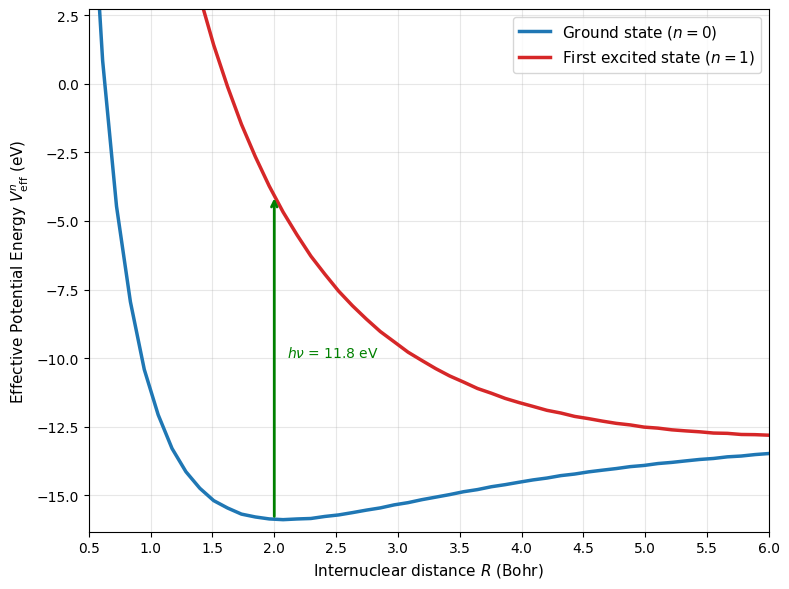
\includegraphics[width=0.9\textwidth]{figures/H2plus effective nuclear potential.png} 
	\caption{Effective nuclear potential energy for $\text{H}_2^+$} 
	\label{fig:H2+ effective nuclear potential} 
\end{figure}
\\The ground state clearly shows a stable bound state when the internuclear distance is $2$ Bohr. For the first excited state the effective potential energy is, by contrast, purely repulsive and there is no stable bound state. In the first excited state the electronic density between the two Hydrogen nuclei drops to zero. Because the Coulomb repulsion between them is not counterbalanced by the electron, the chemical bond between two nuclei is severed, causing them to inevitably go their separate ways.

\subsection{Photo-dissociation energy}
Consider the $\text{H}_2^+$ molecular ion in its ground state ($n=0$). Its electron can be excited to the $n=1$ state by absorbing a photon, which puts the nuclei in an unstable state where each proton is repelled to infinity. The \emph{photo-dissociation energy} needed to break the chemical bond in $\text{H}_2^+$ is shown by the green arrow on figure \ref{fig:H2+ effective nuclear potential}, which corresponds to $11.8$ eV. The same photo-dissociation effect is at play in the first stage of photosynthesis in which photons break water molecules into $\text{H}^+$ ions, free electrons, and release oxygen in the environment.

 \subsection{The physical nature of chemical bonds}
 The electronic wave function provides a perhaps clearer perspective on the stability of the first two energy states of $\text{H}_2^+$. Figure \ref{fig:H2+ electronic wave function} depicts the electronic probability density $|\phi_n(\mathrm{x},R)|^2$ when the internuclear distance is set to two Bohr.
 \begin{figure}[htbp] 
 	\centering
 	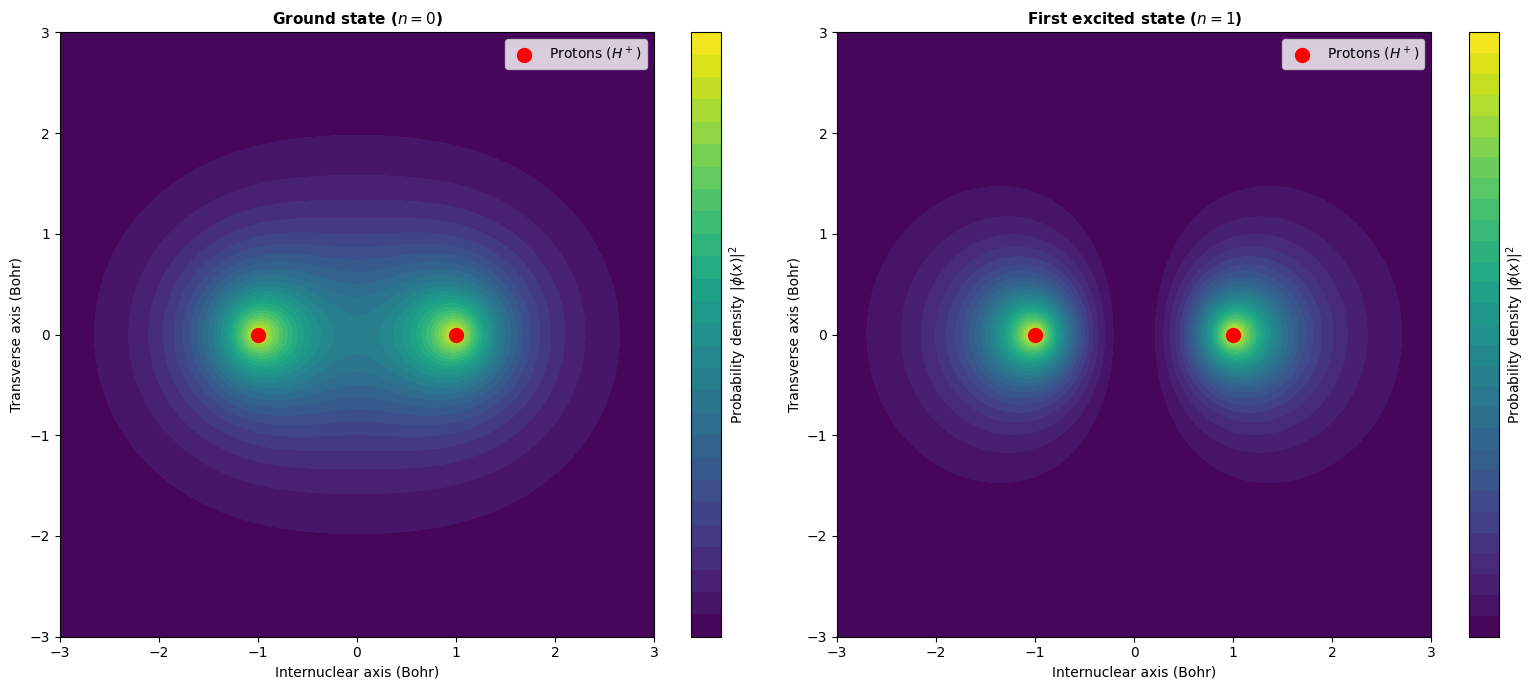
\includegraphics[width=1\textwidth]{figures/Electronic wave function.png} 
 	\caption{Electronic wave function of $\text{H}_2^+$} 
 	\label{fig:H2+ electronic wave function} 
 \end{figure}
\\In the first excited state the electronic density between the two Hydrogen nuclei drops to zero. Because the Coulomb repulsion between them is not counterbalanced by the electron, the chemical bond between two nuclei is severed, causing them to inevitably go their separate ways. In the ground state however, the higher electronic density between the nuclei is enough to keep them bonded. The two nuclei are attracted to the same electron which acts as a \emph{mediator} that tames their mutual repulsion. This is the fundamental physical nature of chemical bonds.
 
\section{Limitations of the Born-Oppenheimer approximation}
\subsection{Electronic energy level crossing}
The Born-Oppenheimer approximation is predicated on the adiabatic theorem, whose central hypothesis is that for two electronic energy eigenstates $m \neq n$ we have
\begin{equation*}
	\langle\phi_m(\mathbf{X}) | \nabla_\alpha |\phi_n(\mathbf{X})\rangle = \frac{\langle\phi_m(\mathbf{X}) | \nabla_\alpha H_{el} | \phi_n(\mathbf{X}) \rangle}{E_n^{el}(\mathbf{X}) - E_m^{el}(\mathbf{X})} \approx 0
\end{equation*}
When dealing with distinct electronic eigenstates such that $E_n^{el}(\mathbf{X}_0) \approx E_m^{el}(\mathbf{X}_0)$ for a given nuclear geometry $\mathbf{X}_0$, the term $\langle\phi_m(\mathbf{X}_0) | \nabla_\alpha |\phi_n(\mathbf{X}_0)\rangle$ diverges and the Born-Oppenheimer approximation breaks down. In this situation the effective nuclear potential energy becomes unphysical. Indeed, looking at equation \eqref{eq:Effective nuclear potential energy}
\begin{equation*}
	V_{\text{eff}}^n(\mathbf{X}) = \frac{e^2}{8\pi\varepsilon_0} \sum_{\alpha \neq \beta} \frac{Z_\alpha Z_\beta}{|\mathbf{X}_\alpha - \mathbf{X}_\beta|} + E_n^{el}(\mathbf{X}) - \sum_\alpha \frac{\hbar^2}{2m_\alpha} \Big(\sum_{l \neq n} |\langle\phi_l(\mathbf{X}_0) | \nabla_\alpha | \phi_n(\mathbf{X}_0)\rangle|^2\Big)
\end{equation*}
we see that if $\langle\phi_m(\mathbf{X}_0) | \nabla_\alpha |\phi_n(\mathbf{X}_0)\rangle$ goes to infinity, so do the $\langle\phi_l(\mathbf{X}_0) | \nabla_\alpha | \phi_n(\mathbf{X}_0)\rangle$ terms which in turn sends $V_{\text{eff}}^n(\mathbf{X}_0)$ to infinity. This nonsensical result at $\mathbf{X}_0$ is merely the price we pay for using the Born-Oppenheimer approximation on a nuclear configuration incompatible with the adiabatic limit.
One solution is to forgo the adiabatic eigenstates in the nuclear configuration region where $E_n^{el}(\mathbf{X})$ and $\approx E_m^{el}(\mathbf{X})$ are getting dangerously closed. The idea is to expand the molecular wave function on an orthonormal basis of \emph{diabatic} states $|\lambda_n\rangle$ which do not depend on the nuclear positions \cite{Smith1969}:
\begin{equation*}
	\Psi(\mathbf{x}, \mathbf{X}) = \sum_n \lambda_n(\mathbf{x}) \chi_n(\mathbf{X})
\end{equation*}
The fact that $\langle\lambda_m | \nabla_\alpha | \lambda_n \rangle = 0$ is precisely why the $\langle\phi_l(\mathbf{X}_0) | \nabla_\alpha | \phi_n(\mathbf{X}_0)\rangle$ terms in the effective nuclear potential energy do not diverge\footnote{When it is not possible to find purely diabatic states with $\nabla_{\alpha}|\lambda_n\rangle = 0$, we instead require that the set of $|\lambda_n\rangle$ vary smoothly and slowly with $\text{X}_{\alpha}$}. The $(m,n)$ element of the electronic Hamiltonian operator written in this diabatic basis is:
\begin{equation*}
	(H_{el}^{\text{dia}}(\mathbf{X}))_{m,n} = \langle\lambda_m | H_{el}(\mathbf{X}) | \lambda_n \rangle
\end{equation*}
This $H_{el}^{\text{dia}}$ is then used to calculate the diabatic energy surfaces $E_{n,dia}^{el}(\mathbf{X})$, and the effective nuclear potential energy in the diabatic basis becomes:
\begin{equation*}
	V_{\text{eff}}^{n,dia}(\mathbf{X}) = \frac{e^2}{8\pi\varepsilon_0} \sum_{\alpha \neq \beta} \frac{Z_\alpha Z_\beta}{|\mathbf{X}_\alpha - \mathbf{X}_\beta|} + E_{n,dia}^{el}(\mathbf{X})
\end{equation*}
\\If we write $[\mathbf{X}_0-\Delta\mathbf{X}\cdots\mathbf{X}_0+\Delta\mathbf{X}]$ the interval\footnote{The term interval is not really appropriate here because the nuclear configuration space is a $3N$ manifold} where the divergence of $\langle\phi_m(\mathbf{X}) | \nabla_\alpha |\phi_n(\mathbf{X})\rangle$ is dangerously close to infinity, the electronic eigenstate basis can be patched up according to the following logic:
\begin{itemize}[]
	\item For $\lVert \mathbf{X} - \mathbf{X}_0 \rVert < \Delta\mathbf{X}$, i.e. inside the degeneracy interval, the \underline{diabatic} basis is used and the effective nuclear potential energy is defined as $V_{\text{eff}}^{n,dia}(\mathbf{X})$
	\item For $\lVert \mathbf{X} - \mathbf{X}_0 \rVert > \Delta\mathbf{X}$, i.e. outside the degeneracy interval, $\Phi(\mathbf{x},\mathbf{X})$ is expanded on the \underline{adiabatic} basis is used and the effective nuclear potential energy is defined as $V_{\text{eff}}^{n,adia}(\mathbf{X})$
\end{itemize}
However, we can't just violently change the basis on which we expand $\Phi(\mathbf{x},\mathbf{X})$ as we move in and out of the degeneracy interval $[\mathbf{X}_0-\Delta\mathbf{X}\cdots\mathbf{X}_0+\Delta\mathbf{X}]$, we run the risk of making $\Phi$ not continuous and differentiable everywhere which is mandatory for a well behaved wave function. Instead we use a unitary operator $U(\mathbf{X})$ to transform one basis into the another, provided that $U(\mathbf{X})$ is continuous and differentiable on the entire nuclear configuration space. Let's look at some of the properties of this unitary transformation operator. We can decompose any adiabatic eigenstate on the basis of diabatic states $|\lambda_k\rangle$:
\begin{equation}
	\label{eq:Adiabatic decomposition}
	|\phi_n(\mathbf{X})\rangle = \sum_k U_{nk}(\mathbf{X})|\lambda_k\rangle
\end{equation}
where $U_{nk}(\mathbf{X})$ is the $(n,k)$ element of our transformation operator $U(\mathbf{X})$. This basis transformation must preserve physical expectations and there must conserve probabilities. This requirement means that the scalar product of $| \phi_n \rangle$ and $| \phi_m \rangle$ must be equal to the scalar product between the transformed vectors $| \lambda_n \rangle$ and $| \lambda_m \rangle$:
\begin{equation*}
	\begin{gathered}
		\langle\phi_m|\phi_n\rangle = \Big(\sum_p U_{mp}|\lambda_p\rangle\Big)^{\dagger} \sum_k U_{nk}|\lambda_k\rangle \\
		\langle\phi_m|\phi_n\rangle = \sum_{p,k} (U_{mp})^{*}U_{nk}\langle\lambda_p|\lambda_k\rangle \\
		\delta_{mn} = \sum_{p,k} U_{nk}(U_{mp})^{*}\delta_{pk} \\
		\delta_{mn} = \sum_p U_{np}(U_{mp})^{*} \\
		\delta_{mn} = \sum_p U_{np}(U^{\dagger})_{pm} \\
		\mathbf{1} = UU^{\dagger}
	\end{gathered}
\end{equation*}
The last equation means that $U(\mathbf{X})$ must be unitary. One way to understand what the elements of $U(\mathbf{X})$ represent is to take the scalar product of equation \eqref{eq:Adiabatic decomposition} with a diabatic state:
\begin{equation*}
	\begin{gathered}
		\langle\lambda_m|\phi_n(\mathbf{X})\rangle = \sum_k U_{nk}(\mathbf{X})\langle\lambda_m|\lambda_k\rangle \\
		\langle\lambda_m|\phi_n(\mathbf{X})\rangle = \sum_k U_{nk}(\mathbf{X})\delta_{mk} \\
		\langle\lambda_m|\phi_n(\mathbf{X})\rangle = U_{nm}(\mathbf{X}) \Leftrightarrow \langle\phi_n(\mathbf{X})|\lambda_m\rangle = U_{nm}(\mathbf{X})^{*}
	\end{gathered}
\end{equation*}
The last equation shows that $U_{nm}(\mathbf{X})$ is the projection of $|\phi_n(\mathbf{X})\rangle$ on $|\lambda_m\rangle$, and $U_{nm}(\mathbf{X})^{*}$ the projection of $|\lambda_m\rangle$ on $|\phi_n(\mathbf{X})\rangle$.
Applying the nuclear gradient operator $\nabla_{\alpha}$ to equation \eqref{eq:Adiabatic decomposition} yields (remember that the diabatic states have the property $\nabla_{\alpha}|\lambda_k\rangle = 0$):
\begin{equation*}
	\begin{gathered}
		\nabla_{\alpha} |\phi_n(\mathbf{X})\rangle = \nabla_{\alpha} \sum_k U_{nk}(\mathbf{X})|\lambda_k\rangle\\
		\nabla_{\alpha} |\phi_n(\mathbf{X})\rangle = \sum_k \nabla_{\alpha}(U_{nk}(\mathbf{X}))|\lambda_k\rangle\\
		\langle\phi_m(\mathbf{X})| \nabla_{\alpha} |\phi_n(\mathbf{X})\rangle = \sum_k \nabla_{\alpha}(U_{nk}(\mathbf{X}))\langle \phi_m(\mathbf{X})|\lambda_k\rangle \\
		\langle\phi_m(\mathbf{X})| \nabla_{\alpha} |\phi_n(\mathbf{X})\rangle = \sum_k \nabla_{\alpha}(U_{nk}(\mathbf{X}))U_{mk}(\mathbf{X})^{*} \\
		\langle\phi_m(\mathbf{X})| \nabla_{\alpha} |\phi_n(\mathbf{X})\rangle = \sum_k \nabla_{\alpha}(U_{nk}(\mathbf{X}))(U^{\dagger})_{km}(\mathbf{X})
	\end{gathered}
\end{equation*}
In matrix form this translates to:
\begin{equation*}
		\mathcal{D}_{\alpha}(\mathbf{X}) = \nabla_{\alpha}(U(\mathbf{X}))U^{\dagger}(\mathbf{X})
\end{equation*}
where  $\mathcal{D}_{\alpha}(\mathbf{X})$ is the matrix representation of the $\nabla_{\alpha}$ operator in the adiabatic basis. Because $U(\mathbf{X})$ is unitary when we multiply both sides by $U(\mathbf{X})$ we get:
\begin{equation*}
	\begin{gathered}
		\mathcal{D}_{\alpha}(\mathbf{X})U(\mathbf{X}) = \nabla_{\alpha}(U(\mathbf{X})) \\
		U(\mathbf{X}) = \exp\Bigg(\int \mathcal{D}_{\alpha}(\mathbf{X}')d\mathbf{X}'\Bigg)
	\end{gathered}
\end{equation*}
The transformation operator $U(\mathbf{X})$ is built as a smooth integral of $\mathcal{D}_{\alpha}(\mathbf{X})$ whose elements are precisely the $\langle\phi_m(\mathbf{X})| \nabla_{\alpha} |\phi_n(\mathbf{X})\rangle$ terms that are diverging inside the degeneracy interval.

\subsection{Beyond single electron molecules}
Another limitation arises for molecules with more than one electron. Although the computation of more complex molecules follows the same underlying principle, having multiple electrons turns the electronic eigenvalue equation into something of a challenge. Even with the simple dihydrogen molecule whose nuclear configuration space is still limited to the internuclear distance, the electronic Hamiltonian becomes:
\begin{equation*}
	\begin{split}
		H_{el} = & \left[ -\frac{\hbar^2}{2m_e} \nabla_1^2 - \frac{e^2}{4\pi\varepsilon_0} \left( \frac{1}{|R_1 - \mathrm{x}_1|} + \frac{1}{|R_2 - \mathrm{x}_1|} \right) \right] \\
		& + \left[ -\frac{\hbar^2}{2m_e} \nabla_2^2 - \frac{e^2}{4\pi\varepsilon_0} \left( \frac{1}{|R_1 - \mathrm{x}_2|} + \frac{1}{|R_2 - \mathrm{x}_2|} \right) \right] \\
		& + \left[ \frac{e^2}{4\pi\varepsilon_0 |\mathrm{x}_1 - \mathrm{x}_2|} \right]
	\end{split}
\end{equation*}
where $\mathrm{x}_1$ and $\mathrm{x}_2$ are the position vectors of electron 1 and 2. The first two brackets are independent: we can solve the first one for $\mathrm{x}_1$ and it won’t affect the second one which only depends on $\mathrm{x}_2$. The rub lies in the third term because it depends simultaneously on both $\mathrm{x}_1$ and $\mathrm{x}_2$. This correlation between the various terms of the electronic Hamiltonian makes it impossible to separate the eigenvalue problem into independent equations. In addition, one has to consider Pauli’s exclusion principle when dealing with multiple electrons because two electrons cannot occupy the same quantum state. As an example, the \emph{Hartree-Fock} method provides a computational framework to find the energy levels of multi-electrons molecules  \cite{Fock1930}.

\begin{thebibliography}{9}
\bibitem{Born1927}
M. Born and R. Oppenheimer, \emph{Zur Quantentheorie der Molekeln}, Annalen der Physik \textbf{389}, 457 (1927).

\bibitem{BornHuang1954}
M. Born and K. Huang, \emph{Dynamical Theory of Crystal Lattices}, Clarendon Press, Oxford (1954).

\bibitem{SzaboOstlund}
A. Szabo and N. S. Ostlund, \emph{Modern Quantum Chemistry: Introduction to Advanced Electronic Structure Theory}, Dover Publications (1996).

\bibitem{Smith1969} F. T. Smith, \emph{Diatomic Interactions and Chemical Bonding. I. Diabatic Representation}, Phys. Rev. \textbf{179}, 111 (1969).

\bibitem{Fock1930} V. Fock, \emph{Näherungsmethode zur Lösung des quantenmechanischen Mehrkörperproblems}, Zeitschrift für Physik \textbf{61}, 126--148 (1930).
\end{thebibliography}
\end{document}
